\section{Allocation Helps, but Selection Dominates the Remaining Gap}
\label{sec:allocation-selection}

\begin{figure}[t]
    \centering
    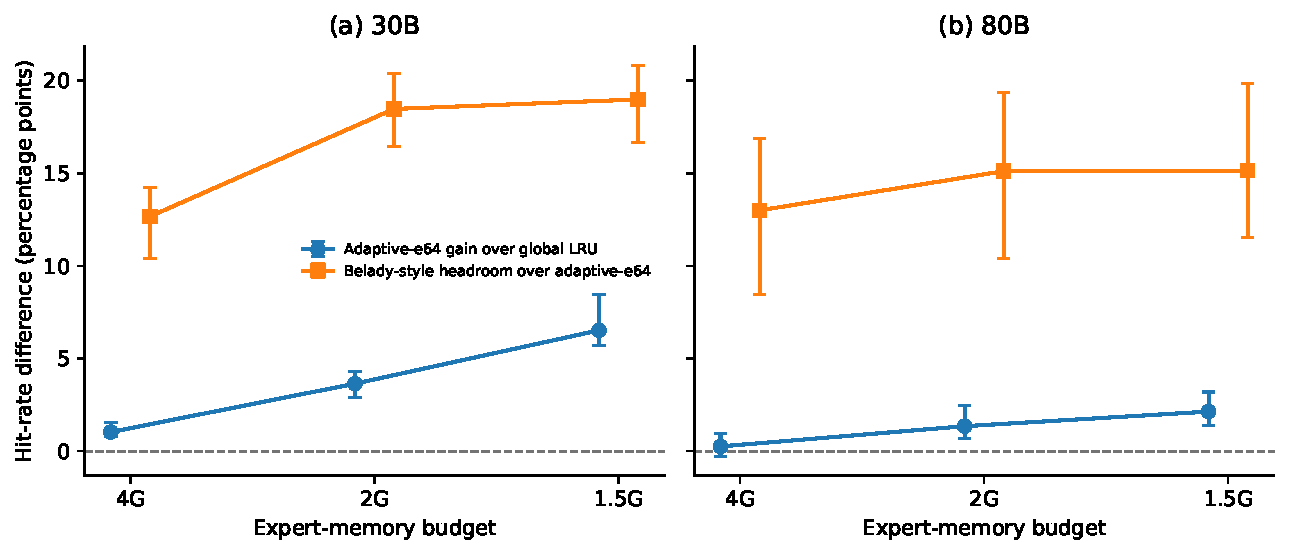
\includegraphics[width=\linewidth]{../experiments/EXP-007-router-characterization/figures/allocation_vs_selection.pdf}
    \caption{Allocation matters, but selection matters more. Median hit-rate improvement of \texttt{adaptive-e64} over global LRU and remaining Belady-style future-informed headroom across the 14 in-sample workload/split cells for each model and memory budget; whiskers show the full observed range. Layer-aware allocation becomes increasingly valuable under stronger memory pressure, especially for the 30B model. Nevertheless, the remaining future-informed selection headroom is substantially larger in every tested model/budget condition. The Belady-style reference is not an achievable online policy and is used only to quantify residual selection opportunity.}
    \label{fig:allocation-selection}
\end{figure}

Layer heterogeneity creates an allocation opportunity, but it does not tell us how much of the total cache-performance gap can be removed by moving capacity between layers. We therefore separate the gain attributable to the tested layer-aware controller from the remaining gain exposed by future-informed expert selection.

Let $h(P)$ denote the replay hit rate of policy $P$ on one trace and budget. Define
\begin{align}
    G_{\mathrm{alloc}}
    &=
    h(\texttt{adaptive-e64})-h(\mathrm{global\ LRU}),
    \label{eq:galloc}\\
    G_{\mathrm{select}}
    &=
    h(\mathrm{Belady})-h(\texttt{adaptive-e64}).
    \label{eq:gselect}
\end{align}
The first quantity asks how much is gained by the tested layer-aware allocation relative to conventional global recency. The second is not an achievable online gain: it measures how much expert-selection opportunity remains if future accesses are known.

\subsection{Allocation becomes more valuable under pressure}

For the 30B, \texttt{adaptive-e64} improves hit rate over global LRU by approximately 0.8--1.5 percentage points at 4\,GiB and 5.7--8.5 points at 1.5\,GiB across the 14 workload/split cells. For the 80B, the corresponding ranges are $-0.3$--$+0.9$ points at 4\,GiB and $+1.4$--$+3.2$ points at 1.5\,GiB. The direction is therefore clearest under stronger pressure, particularly for the 30B.

The gain should not be attributed entirely to rapid adaptation. At 1.5\,GiB, a fixed per-layer partition already captures most of the re-partitioning benefit; relative to that partition, the changing adaptive split adds only about 1.4--1.8 points on the 30B and 0.4--0.7 points on the 80B. Section~\ref{sec:workload-drift} tests the temporal mechanism directly.

Nor is \texttt{adaptive-e64} universally the best online-style replay policy. A 2Q alternative matches or exceeds it at several 80B points, mostly at 4\,GiB. The result of interest is therefore not that one controller dominates the policy space, but that layer-aware partitioning is useful in constrained regimes.

\subsection{The larger gap is within-layer selection}

Figure~\ref{fig:allocation-selection} shows a substantially larger residual gap to the Belady-style future-informed reference. Across the evaluated model/budget conditions, Belady remains approximately 8.5--20.8 percentage points above \texttt{adaptive-e64}. This residual is several times larger than the measured gain from re-splitting memory across layers.

\begin{proposition}[Selection headroom exceeds re-allocation headroom in the evaluated replay]
\label{prop:selection-headroom}
Within the EXP-007 replay abstraction, the remaining future-informed expert-selection headroom after \texttt{adaptive-e64} is larger than the layer-allocation gain recovered over global LRU across the tested model/budget conditions summarized in Figure~\ref{fig:allocation-selection}.
\end{proposition}

\begin{proof}
The ranges are separated in every model/budget group. For the 30B at 4, 2, and 1.5\,GiB, the maximum observed allocation gains are 1.542, 4.314, and 8.461 percentage points, while the minimum future-informed selection headrooms are 10.417, 16.432, and 16.677 points. For the 80B, the corresponding maxima are 0.936, 2.486, and 3.193 points, while the corresponding selection minima are 8.466, 10.394, and 11.552 points. Hence, in each of the six model/budget groups summarized in Figure~\ref{fig:allocation-selection}, even the largest observed re-allocation gain remains below the smallest observed future-informed selection headroom.
\end{proof}

The Belady comparison is intentionally an upper-reference calculation rather than a deployable algorithm. It does not imply that an online predictor can realize the full gap. It instead changes the optimization priority suggested by the data: once layer capacity is partitioned reasonably, the larger measured opportunity lies in deciding \emph{which} experts to retain, not merely in changing \emph{how much} memory each layer receives.
